%!TEX root = ../../PhD_thesis__Edouard_Leurent.tex

\graphicspath{{2-Chapters/1-Chapter/}}

\chapter{Introduction}
\label{chapter:1}

\begin{flushright}
	\begin{tabular}{@{}l@{}}
		\emph{Pour soulever un poids si lourd,}\\
		\emph{Sisyphe, il faudrait ton courage !}\\
		\emph{Bien qu’on ait du cœur à l’ouvrage,}\\
		\emph{L’Art est long et le Temps est court.}\\
	\end{tabular}

	Charles Baudelaire, \href{https://eleurent.github.io/sisyphe/texts/le-guignon.html}{\emph{Le guignon}}.
\end{flushright}

\section{Context and scope}


\subsection{How should a driving robot make decisions?}

In the first few weeks of my PhD, I observed that layman interlocutors, when confronted to this question on the occasion of a social dinner, have a general tendency to conjure up disaster scenarios involving imminent accidents with unavoidable casualties. This reflex is likely to stem from the popularisation of the Trolley Problem \citep{Foot1967}, a famous thought experiment in Moral Philosophy, depicted in \Cref{fig:trolley}, in which a runaway trolley is headed straight toward five people tied up on the main track and unable to move. A lever, when pulled, switches the trolley to a side track occupied by one person: what should you do? Answering this general question of what we \emph{ought} to do in any situation, what is a \emph{right} or \emph{wrong} decision, is the focus of the field of {normative ethics}. This dilemma illustrates a clash between two schools of thought: utilitarianism and deontological ethics. According to utilitarians, the rightfulness of an action should be evaluated based on its consequences, and actions maximising a \emph{utility} --the happiness and well-being for the affected individuals-- should be preferred. Conversely, deontologists evaluate the morality of actions \emph{per se}, according to a series of rules, rather than based on their consequences. Although this problem was initially introduced as a thought experiment, its transposition to the context of autonomous driving and arguably more realistic scenarios made it heavily cited in discussions regarding safety \citep[e.g.][]{Lin2015,Bonnefon2016,Gogoll2017}. In early 2017, MIT’s Media Lab launched the \emph{Moral Machine} platform \citep{Awad2018}, in which members of the public were invited to select the morally acceptable decision out of several options available to an autonomous vehicle. The authors argued that the recovered global preference would provide \emph{"essential topics to be considered by policymakers"}, and \citep{Noothigattu2018} proposed an implementation of a system aggregating these preferences, trained on the collected data. However, the relevance of this analogy to inform engineering and policy has been called into question. Thus, \citet{DeFreitas2019} point out that such dilemma are unlikely to occur on real roads, hard to detect by perception systems and to act upon by control systems, and that they are distracting researchers from the more appropriate goal of how to avoid accidents altogether. Indeed, when we drive we seldom find ourselves in such extreme situations but rather constantly ponder over less tragic questions-- where does this vehicle intend to go? do I have the time to proceed? what is the appropriate speed to drive at right now? The object of this thesis is to artificially reproduce this cognitive process of how to avoid accidents while driving, which is more a technical matter than an ethical one. Still, the Trolley Problem can be seen as a tale: though unrealistic, it reveals and raises a number of legitimate questions.
Should we base driving decisions on a set of rules? And can these rules be learnt, by trial-and-error or by imitation of human drivers? Should we instead make decisions by comparing the utility of possible outcomes, like utilitarians advocate? And if so, how do we choose a good utility? What happens to the Trolley Problem when we add uncertainty? What is the \emph{right} level of caution to take? It would be illusory to pretend that the practical implications of the Trolley Problem can simply be swept aside and entirely replaced by technicality. Throughout this manuscript, we will see that ethical concerns still underpin most assumptions and design choices of safety-critical software.


\begin{figure}[tp]
	\centering
	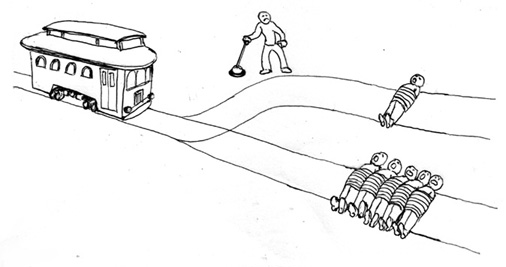
\includegraphics[width=0.7\linewidth]{img/trolley}
	\caption{The Trolley Problem \citep{Foot1967}. Illustration by \href{http://subcortex.com/}{Jesse J. Prinz}.}
	\label{fig:trolley}
\end{figure}

\subsection{Nuts and bolts of self-driving software}

\begin{figure}[th]
	\centering
	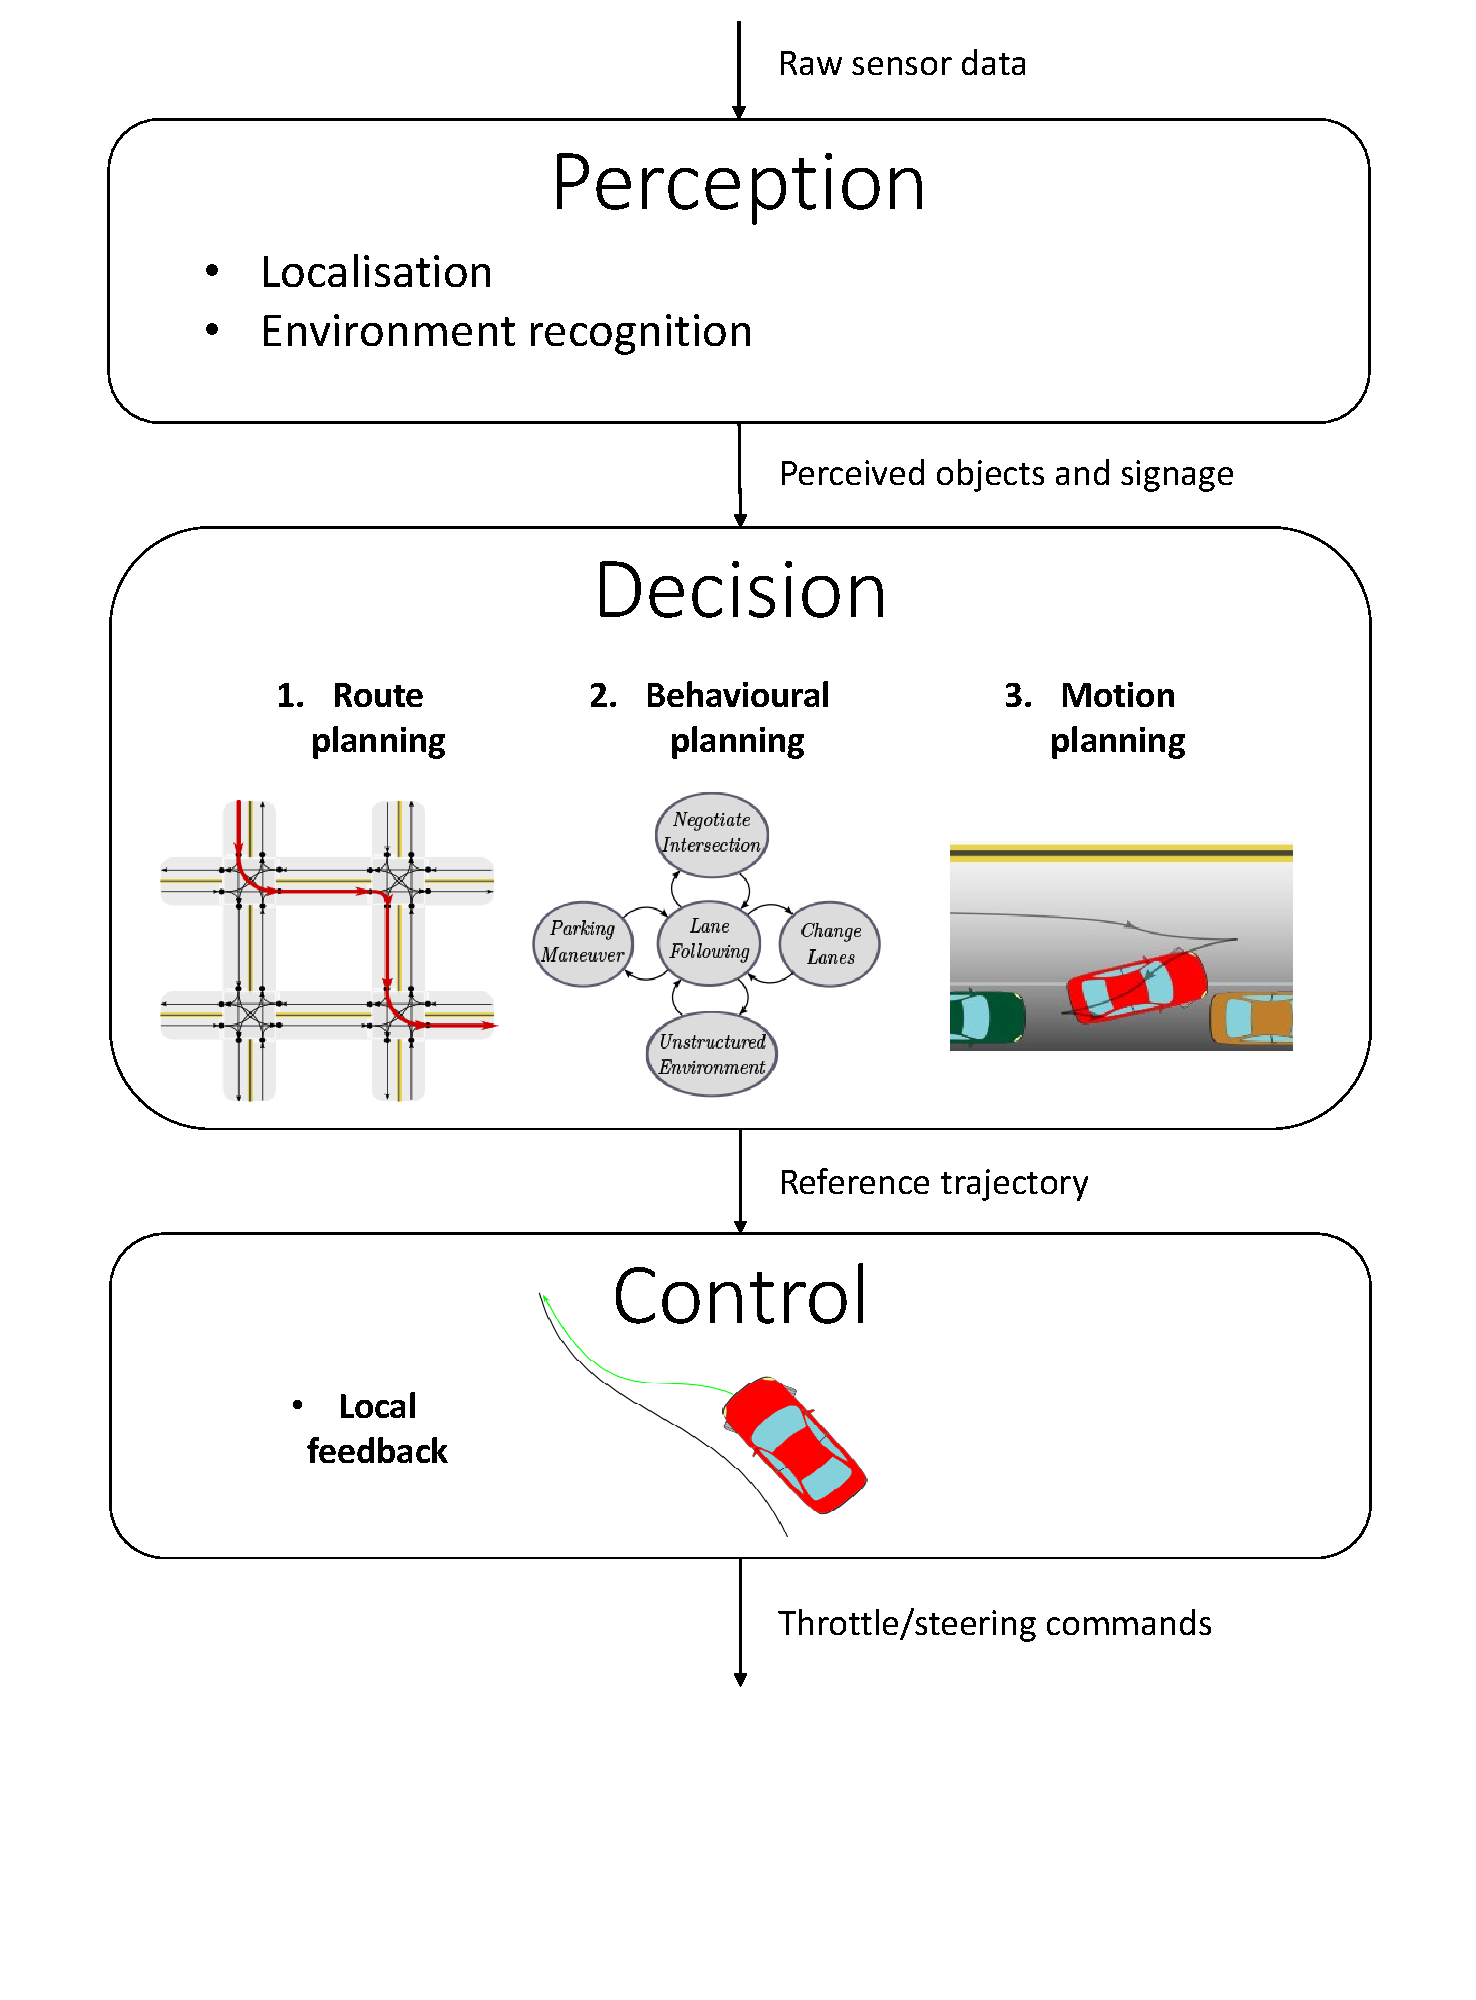
\includegraphics[trim={0 5cm 0 0}, clip, width=0.7\linewidth]{img/pipeline}
	\caption{The architecture of a typical self-driving software}
	\label{fig:robotics-pipeline}
\end{figure}

Historically, autonomous vehicles have been developed by following a traditional robotics pipeline, shown in \Cref{fig:robotics-pipeline}. It involves three main tasks: \emph{Perception}, \emph{Decision}, and \emph{Control} (also called the Sense-Plan-Act paradigm, or Navigation, Guidance and Control in aerospace engineering). The \emph{Perception} module takes raw sensor data as input and produces a high-level reconstruction of the scene. The \emph{Decision} module then determines the desired trajectory of the vehicle, based on the current situation. Finally, the \emph{Control} module manipulates forces, by way of steering and throttle controls, to track the desired trajectory. In the context of Autonomous Driving, the Decision module is often implemented with a hierarchical structure whose layers work at different timescales. First, a \emph{Route Planning} module searches for the shortest route in a road network from the current location to the desires destination. Second, the \emph{Behavioural Planning} layer specifies a coarse driving behaviour through short-term goals or semantic decisions, such as choosing to change lane, to slow down at an intersection, or to yield to a vehicle. This layer is thus responsible for following the planned route while adapting to the current traffic state in real time. Third, the \emph{Motion Planning} layer generates a continuous, feasible trajectory that implements the desired behaviour, while ensuring comfort and safety.

Great strides have been made in the two end-of-pipe tasks: Perception has benefited from the substantial progress in the field of Computer Vision due to the recent advent of Deep Learning, and many control schemes \citep[surveyed in][]{Polack2018} have been developed for ground vehicles. In the Decision module, Route Planning is virtually solved and already provided by services such as \href{https://wiki.openstreetmap.org/wiki/Routing}{Open Street Maps}, and there exist a vast body of Motion Planning algorithms, presented in \Cref{sec:sequential-decision-making}. All these building blocks are widely used in both industrial applications, including \ac{ADAS} functions such as \ac{LKA}, \ac{ACC}, \ac{AEB} or \ac{AES}, and in academic research challenges. Ultimately, we claim that Behavioural Planning remains the only neglected link in the chain. Indeed, most of these applications focused hitherto on simple settings with little complexity: \ac*{ADAS} systems are mostly tailored for highway driving and struggle when merges and interaction. [ref needed]. Similarly, most academic challenges focused on highway driving, with the exception of the DARPA Urban challenge which required more advanced interactions with other vehicles. Yet, even this event still constitutes a controlled environment, simple enough that all participants could rely on rule-based systems for behavioural planning \citep{Buehler2009}, such as finite state machines whose transitions are triggered by handcrafted criteria \citep[\eg][]{Baker2008}. Unfortunately, there is little hope that this approach can scale to complex scenes, since responses tailored for specific use-cases cannot be easily merged together.

\subsection{Scope and Challenges of this Thesis}
\label{sec:scopes-and-challenges}

In the light of the above, this thesis is dedicated to addressing a weak link in the \acl*{AD} chain: \emph{Behavioural Planning}.  We ask the following question: assuming that we had access to a ground truth perception and a perfectly accurate control system, what steps would remain to achieve fully autonomous driving?


\paragraph{Humans in the loop}

In the absence of dedicated self-driving infrastructure, Autonomous Vehicles will have to share the road with human drivers. This introduces a great deal of uncertainty in the decision problem. Indeed, while the location and velocity of a vehicle can be perceived, the mind of its driver remains impenetrable. Even though the present state is known, the future becomes uncertain: where are they headed? Are they paying attention to their surroundings? In that respect, it seems impossible to manually model all the factors involved in the human decision-making process. Yet, human drivers do not drive erratically either. Their behaviour is highly structured: humans drivers tend to follow the lanes, avoid collisions with other vehicles, and generally respect road signage. In other words, human drivers are \emph{predictable}. This motivates the idea of learning from data, and hope for a better comprehensiveness than handcrafted decision systems.%, either direct predictive models of human behaviours, or a driving policy based on implicit predictions of what they might do next.
% We want to quantify uncertainty
% Recall aletoric vs epistemic uncertainty?

\paragraph{Learning to act}

The skill of driving a car involves taking a series of decisions, where early stages influence the resulting outcomes and subsequent reasoning at late stages. This aspect is known as sequential (or multistage) decision-making. Let us start by introducing some useful notations. At each time step $t$, the system is described by its \emph{state} $s_t$ that belongs to a measurable state space $\cS$. Then, the agent can take an \emph{action} $a_t$ within a measurable action space $\cA$, before transitioning to a next state $s_{t+1}\in\cS$, drawn from a conditional distribution $P\parentheses{s_{t+1} \mid s_t, a_t}$ that we call the \emph{system dynamics}. The agent actions can themselves be drawn from a distribution $\pi\parentheses{a_t\mid s_t}$, called the \emph{policy}.

\ac{RL} is a general framework for learning-based sequential decision-making. It is formulated as an optimal control problem: the policy $\pi$ is chosen to maximise an objective function. It is generally formalized as a \ac{MDP}, \ie a tuple $(\cS, \cA, P, R, \gamma)$ in which at each step $t$, a bounded reward $r_t\in[0, 1]$ drawn from a reward distribution $R(r_t|s_t,a_t)$. The agent must act so as to optimise in expectation its cumulative discounted reward, also called \emph{return}, where $\gamma\in[0,1)$ is the discount factor:

\begin{equation*}
V^*(s) = \max_{\pi}V^\pi(s),\, \text{ where } V^\pi(s) = \expectedvalue_{\pi, P} \left[\sum_t \gamma^t r_t\condbar s_0 = s\right].
\end{equation*}

Several performance measures have been introduced to evaluate \ac*{RL} algorithms. In this thesis, we consider the goal of finding a near-optimal policy as fast as possible. In the \emph{fixed-confidence} setting, the goal is to find a near-optimal policy $\pi^*$ with high probability with the smallest required sample complexity, \ie number of interactions. Alternatively, in the \emph{fixed-budget} setting, the \emph{simple regret} $r_n$ of an algorithm measures the \emph{expected} sub-optimality of the recommenced policy $\hat{\pi}_n$ after a fixed number $n$ of interactions.
\begin{equation*}
r_n(s) = \expectedvalue_{\hat{\pi}_n} \left[ V^\star(s) - V^{\hat{\pi}}(s) \right]
\end{equation*}

%Conversely, in real environments where exploration is costly, another objective is to minimise the \textit{cumulative regret}.
%\begin{equation*}
%\cR_n(s_0, \cA) = \expectedvalue_{\hat{\pi}_t\sim \cA}\left[ \sum_{t=0}^{n-1} V^\star(s_t) - V^{\hat{\pi}_t}(s_t) \right]
%\end{equation*}

The first goal of this thesis is to provide \emph{sample-efficient} algorithms for learning a driving policy. In the particular context of Behavioural Planning for Autonomous Driving, this goal will be articulated around three main questions and challenges.

\paragraph{Model-free \vs model-based}

\ac*{RL} algorithms can be grouped into two main families. 
In order to find an optimal policy $\pi^*$, \emph{Model-based} \ac*{RL} algorithms first attempt to estimate the \ac*{MDP} parameters $\hat{P}$ and $\hat{R}$ based on a history of transitions $\cD = \{(s_{t},a_t, r_t, s_{t+1})\}$, using for instance \ac{MLE} in a hypothesis class of dynamics and reward distributions.
\begin{equation*}
\max_{\hat{P}} \sum_{t}\hat{P}\parentheses{s_{t+1} \mid s_t,a_t} \quad \text{and} \quad \max_{\hat{R}} \sum_{t}\hat{R}\parentheses{r_{t} \mid s_t,a_t}
\end{equation*}
This allows to \emph{plan} in the estimated \ac*{MDP} $(S,A,\hat{R}, \hat{P}, \gamma)$, i.e. compute the associated optimal policy $\hat{\pi}^\star$. Conversely, \emph{Model-free} \ac*{RL} algorithms do not estimate the underlying \ac*{MDP} and aim instead to optimise a policy $\pi$ directly. This often involves an \emph{evaluation} step, where the state value function $V^\pi$, or state-action value function
\begin{equation*}
Q^\pi(s,a) = \expectedvalue_{\pi, P} \left[\sum_t \gamma^t r_t\condbar s_0 = s, a_0 = a\right]
\end{equation*}
are estimated, and an \emph{improvement} step, where the policy $\pi$ is updated to maximise $V^\pi$.

The question of which approach is better depends on the underlying problem. Indeed, the model-based approach is relevant when the dynamics are simple but the optimal policy is complex. For instance, the case of Computer Go was tackled in AlphaGo \citep{Silver2016,Silver2017,Silver2018} with a \ac{MCTS} planning module, which leveraged the knowledge of the Go dynamics (placing pawns on the board) to sample sequences of moves online. On the contrary, the model-free approach is useful when the system dynamics are complex, but the optimal policy is simpler. Thus, a swimming robot would require heavy fluid dynamics simulation to accurately predict the effect of moving its fins, while a simple periodic gait could suffice to propel it forward in water. Which brings us to the question: which scenario does Autonomous Driving fall into? Unfortunately, the answer is not so clear-cut. On one hand, the motion planning literature has historically been heavily relying on kinematics and dynamics models to plan trajectories, as will be detailed in \Cref{chapter:2}. Reliable priors are available to describe the physics of a vehicle, but not so much for the intents of its driver. On the other hand, automotive companies such as Mobileye reportedly\footnote{these comments are reported from discussions between Renault and Mobileye} advocated that the task of predicting a driving scene is actually more difficult than driving properly. The case of Autonomous Driving is actually peculiar in that the two problems of prediction and control are somehow equivalent, due to the presence of other drivers: a good trajectory predictor can be applied to predict the action that a human would do in place of the ego-vehicle, and a good driving policy can be applied to each agent in the scene to produce reasonable trajectories. Hence, both approaches seem relevant and are considered in this thesis.

\paragraph{Social interactions and coupled dynamics}

Conservative behaviours struggle when interacting with other vehicles, a task often referred to as \emph{negotiation}. Scenarios of unprotected left-turns, intersections, or merging onto a highway (see \eg \href{%https://twitter.com/nitguptaa/status/990683818825736192
	https://www.youtube.com/watch?v=HjtiiGCe1pE}{this video} where a Waymo car fails to merge). Other example: the freezing robot.
Thus, for an autonomous vehicle to efficiently integrate with the traffic flow, it must anticipate the effect of its own actions on the behaviours of other agents. This skill is known as \emph{socially-aware} decision-making. Unfortunately, these interactions between vehicles translates as complex and coupled traffic dynamics. Local deviations must be propagated from one vehicle to the next, which can result in a quick and chaotic build-up of uncertainty. We will need to contain this build up of uncertainty, and prevent instability. On the other hand, researchers claim that the task of predicting is actually harder to that of driving properly.

\paragraph{Safety and efficiency}

The complexity of human driving behaviours lead us to consider learning algorithms. However, the use of these methods typically raises a legitimate concern of car manufacturers: how to guarantee the \emph{safety} of such systems, in the presence of uncertainty? In this thesis, we will strive to formalize this concern by formalising different notions of \emph{risk}, as functions of the distribution of outcomes induced by a policy. \emph{Safe} \acl*{RL} seeks to estimate and control the level of risk taken by a policy.
However, protecting against risk often comes at the price of efficiency in achieving a goal. Indeed, the two objectives of driving fast and safely are contradictory. This induces a trade-off that is typically observed in human drivers, especially in situations of negotiations: some people adopt \emph{aggressive} behaviours and try to force their way through traffic, while others act more \emph{defensively}, favouring safety. This trade-off is difficult to capture manually when defining the desired objective of an autonomous vehicle, and soon leads to the pitfall of reward engineering.

\section{Outline and Contributions}

\begin{figure}[ht]
	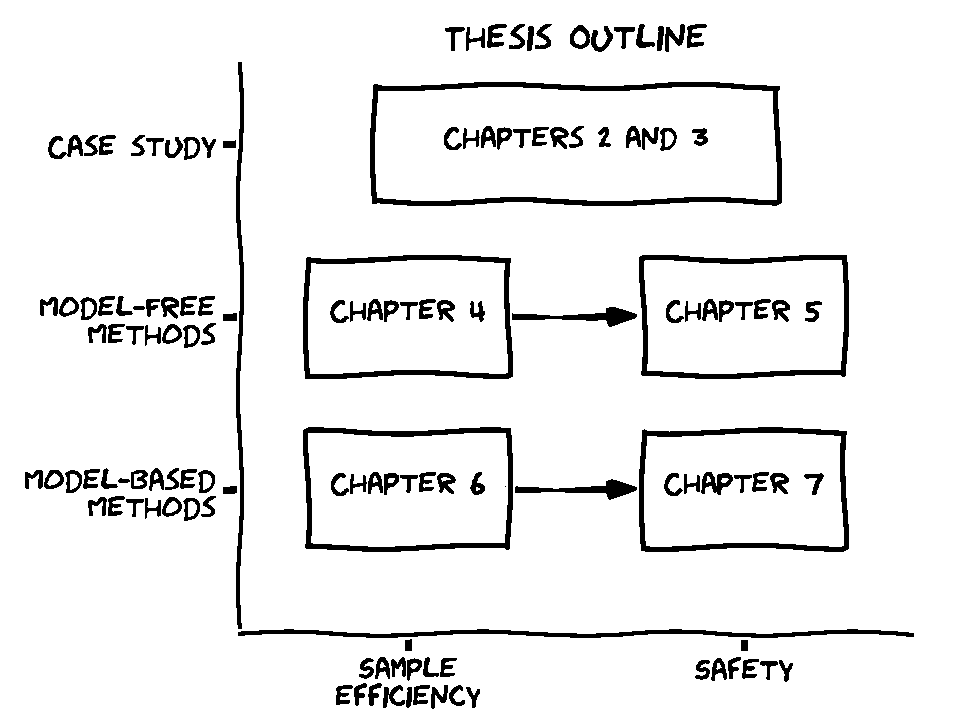
\includegraphics[width=0.9\linewidth]{img/outline}
	\caption{The thesis is structures around two disjunctions: model-free \vs model-based on one hand, and sample-efficiency \vs safety on the other hand.}
	\label{fig:thesis-outline}
\end{figure}

% Part I
The ultimate goal of this thesis could be summarized in the following question: \emph{"how can an algorithm learn to drive and avoid accidents?"}. The first step in such an endeavour must necessarily be to formalize more precisely the meaning of this ill-posed formula, and so we try in \Cref{part:1}.

It is only natural that we begin this journey by turning to the standard model for sequential decision making: the \acl*{MDP}. At first glance, this framework shines with its simplicity and elegance, but also its apparent generality and representation power. Yet, as we embark on the ambitious task of casting the blurry problem of autonomous driving into this rigid mould, we highlight in \Cref{chapter:2} how reductive each step of the formalization is, how approximations and assumptions always hide behind each symbol and each equation. This observation is supported by the numerous variations of the framework that have been developed by the research community, in as many attempts to address these concerns. Such limitations are as varied as partial observability, temporal abstraction, the reward hypothesis, transfer from simulation to real-world and safety; and we relate these research directions to specific works in the autonomous driving literature.

In order to progress, we put aside some of these questions in \Cref{chapter:3} and commit to an (observable) state space, a (hierarchical) action space, a (quasi-linear) system dynamics and a (dense) reward function that we deem suitable for a class of behavioural planning tasks. This allows us to refocus on two fundamental issues: \textit{sample-efficient} and \textit{safe} \acl*{RL}. In the sequel, we tackle them through the perspective of the two main approaches to \acl*{RL} aforementioned: first model-free, and then model-based algorithms.

% Part II
\Cref{part:2} is dedicated to the study of how model-free methods can be applied in the context of autonomous driving. In \Cref{chapter:4}, we question the choice of state representation and model architecture in relation to its associated sample-efficiency. In particular, we identify a few desirable properties and inductive biases, mainly that of \emph{permutation invariance} regarding the observed vehicles in the scene. We propose an attention-based architecture that fulfils our wishes, and compare it to standard representations and architectures that have been used for behavioural planning tasks. 

In \Cref{chapter:5}, \dots 

% Part III
\Cref{part:3} is \dots

In \Cref{chapter:6}, \dots 

In \Cref{chapter:7}, \dots

\subsection*{List of publications}

\subsubsection*{Publications in international conferences with proceedings}

\begin{itemize}
	\item \bibentry{Leurent2019interval} (used in \Cref{chapter:7})
	\item \bibentry{Leurent2020practical} (used in \Cref{chapter:6})
	\item \bibentry{CarraraLeurent2019} (used in \Cref{chapter:5})
\end{itemize}

\subsubsection*{Workshop presentations in international conferences}

\begin{itemize}
	\item \bibentry{Leurent2019social} (used in \Cref{chapter:4})
	\item \bibentry{Leurent2018approximate} (used in \Cref{chapter:7})
\end{itemize}

\subsubsection*{Submitted works}

\begin{itemize}
	\item Robust-Adaptive Control of Linear Systems: beyond Quadratic Costs (used in \Cref{chapter:7})
	\item Robust-Adaptive Interval Predictive Control for Linear Uncertain Systems (used in \Cref{chapter:7})
	\item Monte-Carlo Graph Search: the Value of Merging Similar States (used in \Cref{chapter:6})
\end{itemize}

\subsubsection*{Collaborations not presented in this thesis}

\begin{itemize}
	\item \bibentry{jonsson2020planning}
	\item \bibentry{kaufmann2020adaptive}
\end{itemize}